% Options for packages loaded elsewhere
\PassOptionsToPackage{unicode}{hyperref}
\PassOptionsToPackage{hyphens}{url}
%
\documentclass[
]{article}
\usepackage{amsmath,amssymb}
\usepackage{iftex}
\ifPDFTeX
  \usepackage[T1]{fontenc}
  \usepackage[utf8]{inputenc}
  \usepackage{textcomp} % provide euro and other symbols
\else % if luatex or xetex
  \usepackage{unicode-math} % this also loads fontspec
  \defaultfontfeatures{Scale=MatchLowercase}
  \defaultfontfeatures[\rmfamily]{Ligatures=TeX,Scale=1}
\fi
\usepackage{lmodern}
\ifPDFTeX\else
  % xetex/luatex font selection
\fi
% Use upquote if available, for straight quotes in verbatim environments
\IfFileExists{upquote.sty}{\usepackage{upquote}}{}
\IfFileExists{microtype.sty}{% use microtype if available
  \usepackage[]{microtype}
  \UseMicrotypeSet[protrusion]{basicmath} % disable protrusion for tt fonts
}{}
\makeatletter
\@ifundefined{KOMAClassName}{% if non-KOMA class
  \IfFileExists{parskip.sty}{%
    \usepackage{parskip}
  }{% else
    \setlength{\parindent}{0pt}
    \setlength{\parskip}{6pt plus 2pt minus 1pt}}
}{% if KOMA class
  \KOMAoptions{parskip=half}}
\makeatother
\usepackage{xcolor}
\usepackage[margin=1in]{geometry}
\usepackage{color}
\usepackage{fancyvrb}
\newcommand{\VerbBar}{|}
\newcommand{\VERB}{\Verb[commandchars=\\\{\}]}
\DefineVerbatimEnvironment{Highlighting}{Verbatim}{commandchars=\\\{\}}
% Add ',fontsize=\small' for more characters per line
\usepackage{framed}
\definecolor{shadecolor}{RGB}{248,248,248}
\newenvironment{Shaded}{\begin{snugshade}}{\end{snugshade}}
\newcommand{\AlertTok}[1]{\textcolor[rgb]{0.94,0.16,0.16}{#1}}
\newcommand{\AnnotationTok}[1]{\textcolor[rgb]{0.56,0.35,0.01}{\textbf{\textit{#1}}}}
\newcommand{\AttributeTok}[1]{\textcolor[rgb]{0.13,0.29,0.53}{#1}}
\newcommand{\BaseNTok}[1]{\textcolor[rgb]{0.00,0.00,0.81}{#1}}
\newcommand{\BuiltInTok}[1]{#1}
\newcommand{\CharTok}[1]{\textcolor[rgb]{0.31,0.60,0.02}{#1}}
\newcommand{\CommentTok}[1]{\textcolor[rgb]{0.56,0.35,0.01}{\textit{#1}}}
\newcommand{\CommentVarTok}[1]{\textcolor[rgb]{0.56,0.35,0.01}{\textbf{\textit{#1}}}}
\newcommand{\ConstantTok}[1]{\textcolor[rgb]{0.56,0.35,0.01}{#1}}
\newcommand{\ControlFlowTok}[1]{\textcolor[rgb]{0.13,0.29,0.53}{\textbf{#1}}}
\newcommand{\DataTypeTok}[1]{\textcolor[rgb]{0.13,0.29,0.53}{#1}}
\newcommand{\DecValTok}[1]{\textcolor[rgb]{0.00,0.00,0.81}{#1}}
\newcommand{\DocumentationTok}[1]{\textcolor[rgb]{0.56,0.35,0.01}{\textbf{\textit{#1}}}}
\newcommand{\ErrorTok}[1]{\textcolor[rgb]{0.64,0.00,0.00}{\textbf{#1}}}
\newcommand{\ExtensionTok}[1]{#1}
\newcommand{\FloatTok}[1]{\textcolor[rgb]{0.00,0.00,0.81}{#1}}
\newcommand{\FunctionTok}[1]{\textcolor[rgb]{0.13,0.29,0.53}{\textbf{#1}}}
\newcommand{\ImportTok}[1]{#1}
\newcommand{\InformationTok}[1]{\textcolor[rgb]{0.56,0.35,0.01}{\textbf{\textit{#1}}}}
\newcommand{\KeywordTok}[1]{\textcolor[rgb]{0.13,0.29,0.53}{\textbf{#1}}}
\newcommand{\NormalTok}[1]{#1}
\newcommand{\OperatorTok}[1]{\textcolor[rgb]{0.81,0.36,0.00}{\textbf{#1}}}
\newcommand{\OtherTok}[1]{\textcolor[rgb]{0.56,0.35,0.01}{#1}}
\newcommand{\PreprocessorTok}[1]{\textcolor[rgb]{0.56,0.35,0.01}{\textit{#1}}}
\newcommand{\RegionMarkerTok}[1]{#1}
\newcommand{\SpecialCharTok}[1]{\textcolor[rgb]{0.81,0.36,0.00}{\textbf{#1}}}
\newcommand{\SpecialStringTok}[1]{\textcolor[rgb]{0.31,0.60,0.02}{#1}}
\newcommand{\StringTok}[1]{\textcolor[rgb]{0.31,0.60,0.02}{#1}}
\newcommand{\VariableTok}[1]{\textcolor[rgb]{0.00,0.00,0.00}{#1}}
\newcommand{\VerbatimStringTok}[1]{\textcolor[rgb]{0.31,0.60,0.02}{#1}}
\newcommand{\WarningTok}[1]{\textcolor[rgb]{0.56,0.35,0.01}{\textbf{\textit{#1}}}}
\usepackage{graphicx}
\makeatletter
\def\maxwidth{\ifdim\Gin@nat@width>\linewidth\linewidth\else\Gin@nat@width\fi}
\def\maxheight{\ifdim\Gin@nat@height>\textheight\textheight\else\Gin@nat@height\fi}
\makeatother
% Scale images if necessary, so that they will not overflow the page
% margins by default, and it is still possible to overwrite the defaults
% using explicit options in \includegraphics[width, height, ...]{}
\setkeys{Gin}{width=\maxwidth,height=\maxheight,keepaspectratio}
% Set default figure placement to htbp
\makeatletter
\def\fps@figure{htbp}
\makeatother
\setlength{\emergencystretch}{3em} % prevent overfull lines
\providecommand{\tightlist}{%
  \setlength{\itemsep}{0pt}\setlength{\parskip}{0pt}}
\setcounter{secnumdepth}{-\maxdimen} % remove section numbering
\ifLuaTeX
  \usepackage{selnolig}  % disable illegal ligatures
\fi
\usepackage{bookmark}
\IfFileExists{xurl.sty}{\usepackage{xurl}}{} % add URL line breaks if available
\urlstyle{same}
\hypersetup{
  pdftitle={Lab 1: Introduction to R and RStudio},
  hidelinks,
  pdfcreator={LaTeX via pandoc}}

\title{Lab 1: Introduction to R and RStudio}
\author{}
\date{\vspace{-2.5em}}

\begin{document}
\maketitle

\subsubsection{Instructions}\label{instructions}

\begin{itemize}
\tightlist
\item
  Due date: Monday, July 6th at 11:59pm (Submit via Gradescope, see
  instructions at the bottom of this file)
\item
  Late penalty: 50\% late penalty if submitted within 24 hours of due
  date, no marks for assignments submitted thereafter.
\item
  This assignment is graded on \textbf{correct completion}, all or
  nothing. You must pass all public tests and submit the assignment for
  credit.
\item
  Submission process: Follow the submission instructions on the final
  page. Make sure you do not remove any \texttt{\textbackslash{}newpage}
  tags or rename this file, as this will break the submission.
\end{itemize}

\subsubsection{Welcome to PH142!}\label{welcome-to-ph142}

This year, we've revamped the course to incorporate more of the everyday
data science skills and more time for you to practice using these
skills. We will be using R, a statistical programming language,
throughout this course and other courses offered by the School of Public
Health.

\subsubsection{What is R?}\label{what-is-r}

\begin{itemize}
\tightlist
\item
  R is a programming language. We will use it to manipulate, visualize,
  and analyze data.
\item
  If you've never programmed before, that is okay. We will teach you the
  basics and ensure you know how to do everything you need to know for
  this course. You'll also be using R in PH250A, among other courses.
\end{itemize}

\subsubsection{Why program in R?}\label{why-program-in-r}

\begin{itemize}
\item
  Because it is programming, you can easily save all your steps

  \begin{itemize}
  \tightlist
  \item
    Easy to re-run/duplicate.
  \item
    Easy to extend.
  \end{itemize}
\item
  R is free and open source. This means that anyone can install and use
  it, making it more accessible than SAS and Stata.
\item
  R is flexible and ever-evolving.
\end{itemize}

\subsubsection{What is RStudio?}\label{what-is-rstudio}

RStudio is an integrated development environment (IDE). RStudio makes it
easier to program in R. Without RStudio, all we would see when we open R
is a console where we enter our lines of code.

\subsubsection{Getting up and running in
RStudio}\label{getting-up-and-running-in-rstudio}

By default, RStudio displays four panes shown below:

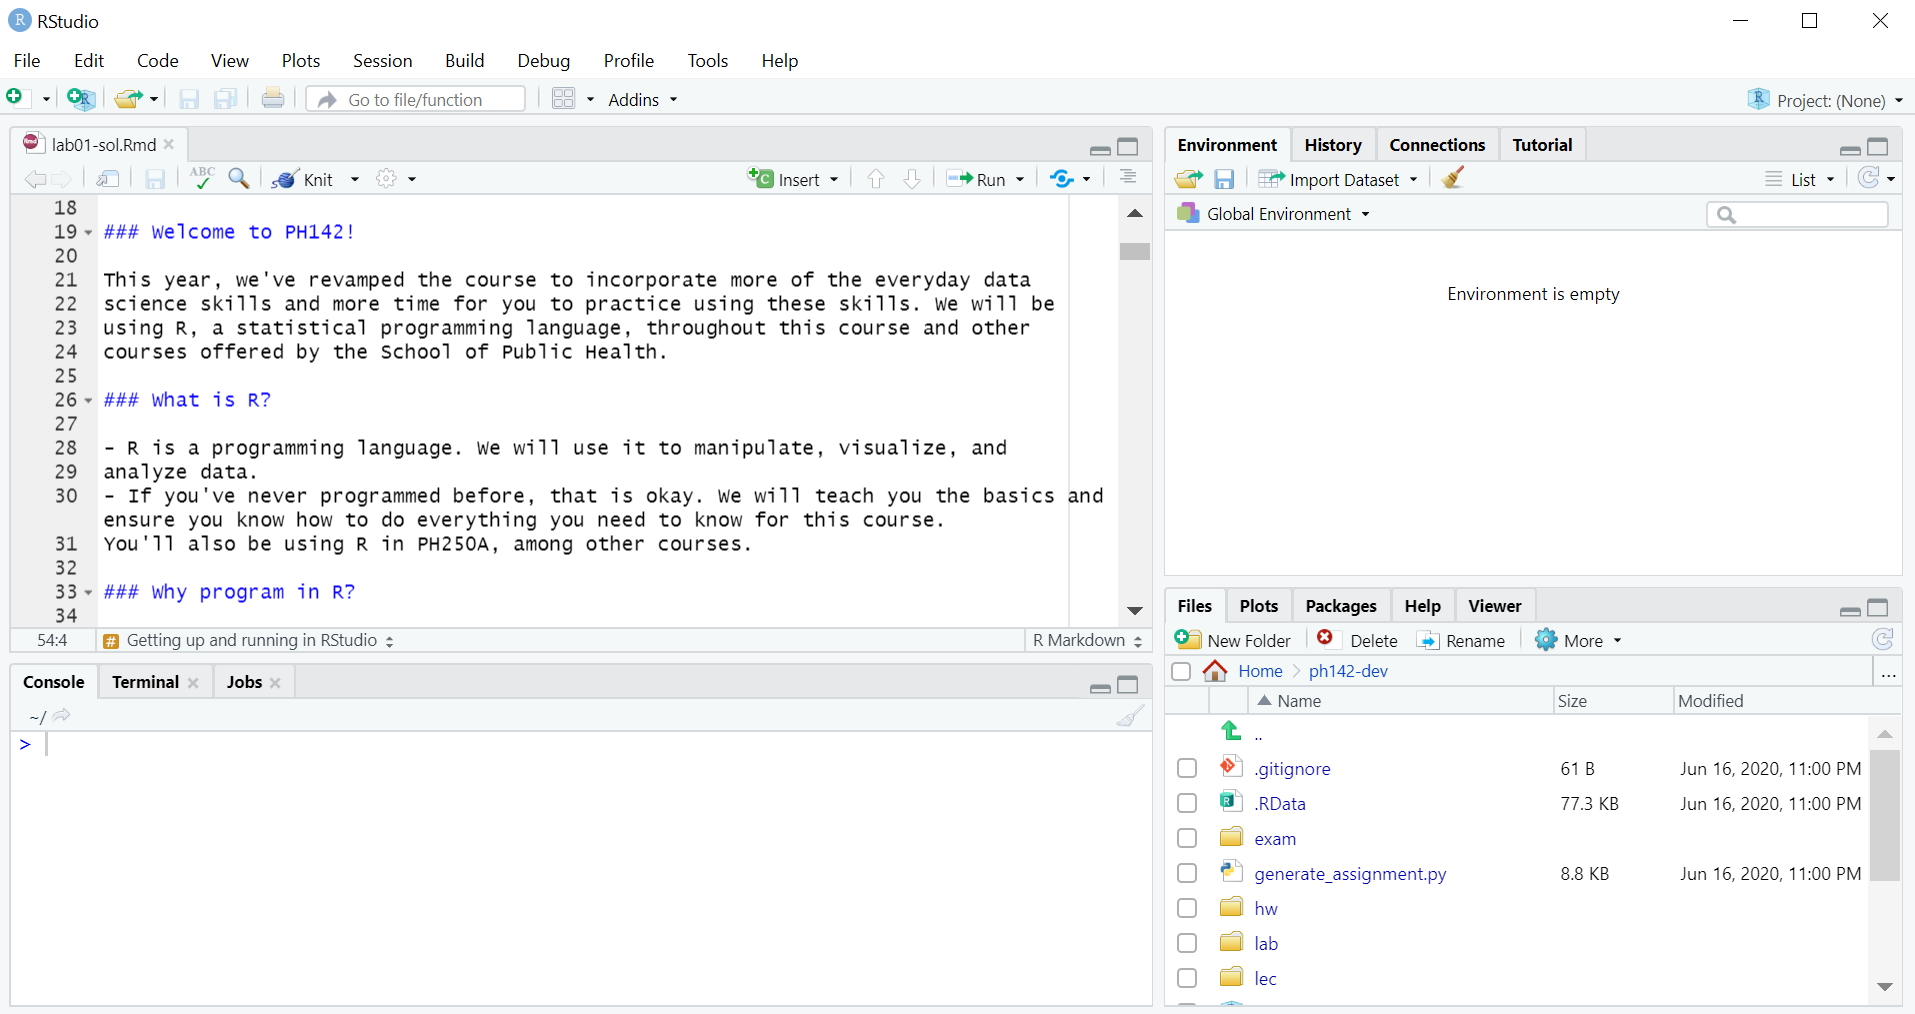
\includegraphics[width=400px]{src/lab01-rstudio-panes}

Today, you will complete the exercises below to become familiar with the
four panes.

\textbf{Pane 1. Console (bottom left pane)} This is where you input code
to be processed. Numeric output will display in the console.

In the console you will notice a \textbf{\textgreater{}} at the
beginning of a line. This is a prompt - it is R's way of saying that it
is your turn to say something. When you type something and press enter,
R will evaluate what you have ``said'' and respond. If you type a number
and hit enter, R will return that number. You can also type an equation
or use R like a calculator.

\begin{itemize}
\tightlist
\item
  \textbf{Exercise 1:} Practice using the console like a calculator.
  Click inside the console, type \texttt{2+2} and hit enter. Make sure
  you can add (+), subtract (-), multiply (*), divide (/), and take
  powers (\^{}). Use round brackets for PEMDAS.
\item
  \textbf{Exercise 2:} Type \texttt{tinytex::install\_tinytex()} in the
  console and press enter. This loads a package that will help you knit
  files more quickly!
\item
  \textbf{Exercise 3:} Suppose you were interested in calculating how
  much you'd earn in a month at a new job. The job pays \$20 per hour
  and you will work 15 hours per week, but are taxed at 20\%. How much
  money after tax will you have at the end of one month? Using the
  console like a calculator, calculate your answer.
\end{itemize}

\textbf{Creating an object} If you would like to save something (a
number, a vector, a dataset etc.) for use later, you can save it as an
object. You can think of this like creating a jar and giving it a label.

For example, type the code \texttt{a\ \textless{}-\ 2} into the console.
This stores the value \texttt{2} in the object \texttt{a}. You can also
type \texttt{a\ \textless{}-\ 1\ +\ 1}, and this does the same thing,
since the evaluation of the right-hand side happens before it is
assigned to the variable. Notice that when you create an object, R does
not respond, but if you then type the object name, R will respond with
the contents of the object.

\textbf{Code chunks} We will often provide code chunks in the R markdown
files: these are little sections of code set off from the text of the
file with \texttt{\{r\}\ at\ the\ beginning\ and} at the end. In Rstudio
you can see that the code chunks appear in a gray background. You should
also notice the green arrows in the upper right hand side of each chunk.
If you click the arrow pointing to the right, R will submit everything
in the ``chunk'' and you will see the results just below the chunk.

\begin{itemize}
\tightlist
\item
  \textbf{Exercise 4:} In the code chunk below, use the assignment
  operator (\texttt{\textless{}-}) to store your answer in an object
  called \texttt{monthly\_wage}. When assigning variables, the stuff on
  the right-hand side of the arrow \texttt{\textless{}-} is evaluated
  first, and then assigned to the object specified by the variable name
  on the left of the arrow.
\end{itemize}

\begin{Shaded}
\begin{Highlighting}[]
\NormalTok{monthly\_wage }\OtherTok{\textless{}{-}} \StringTok{"YOUR CODE HERE"}
\end{Highlighting}
\end{Shaded}

You can also save a series of numbers in an object. For example:
\texttt{heights\ \textless{}-\ c(5,6,2,9,6)} will save a set of values
in the object ``heights''. The \texttt{c()} tells R to ``combine'' the
numbers into a list, known in R as a \textbf{vector}.

\textbf{Pane 2. Environment/History/Connections:} What is in the
environment tab right now? It is letting you know about the
\textbf{objects} that we saved in the \textbf{Environment}. When we load
in a data set, we will also be able to see its object here too. For
datasets, there is an icon we can push to view all the data. Now click
the History tab. What is it? Click a line of code and hit the ``To
Console'' or ``To Source'' buttons. What happens? The History tab is a
great way to recall a line of code that you may have typed directly in
the console but hadn't saved in the code editor and would like to use
again. We will ignore the connections tab.

If you ran the code chunk above, you should see \texttt{monthly\_wage}
as an object in the Environment window.

\textbf{Types of variables in R} Notice in the Environment tab that you
can see a description of each object that has been saved.\\
For datasets, you will see the number of observations and variables. For
variables you will see the type of variable.

In R, continuous variables will be called numeric or ``NUM''.

Categorical variables may be recorded as text or as numbers (category 1,
2, 3 etc.).

Text variables will be called character or ``chr''.

\textbf{Functions} A function is an instruction or a set of instructions
in R. For example sqrt() is a function built in to R. This will take the
square root of a number. Type \texttt{sqrt(81)} into your command
window. In this example: -\textbf{sqrt} is the name of the function:
taking the square root -\textbf{the parentheses} creates a space where
we put the number we want to use the function on -\textbf{81} the number
we are placing in our function There are many functions built in to R.
For example: abs() takes the absolute value log() takes the natural log
exp() gives powers of e ls() will give you a list of all of the objects
in your environment

\subsubsection{Help!}\label{help}

Each function comes with a help page telling you what it does and what
arguments you need to provide the function. There are two ways to see
the help page of a function:

\begin{Shaded}
\begin{Highlighting}[]
\FunctionTok{help}\NormalTok{(}\StringTok{"library"}\NormalTok{)}
\NormalTok{?library}
\end{Highlighting}
\end{Shaded}

When we execute either of the above lines of code, the Help tab will
open and navigate to the help page for the function \texttt{library()}.
Calling a help page in this way is most useful if you know the name of
the function you'd like to use but forget exactly how to use the
function. Don't worry if you can't understand what is written there
right now.

If you would like help, but can't remember then name of the function you
need help with, you can type a double question mark before a word that
is related to the function you are looking for:

\begin{Shaded}
\begin{Highlighting}[]
\NormalTok{??histogram}
\end{Highlighting}
\end{Shaded}

This shows you all the packages and their functions which discuss
histograms. For example \texttt{ggplot2::geom\_freqpoly} means that
there is a function \texttt{geom\_freqpoly()} from the \texttt{ggplot2}
package that is used to make histograms. You can click through the
functions until you find the one you're looking for.

\textbf{Pane 3. Source (top left pane)} a.k.a the code editor a.k.a the
script editor. While the \textbf{console} is meant to be used
interactively, the \textbf{source} is a place to store multiple lines of
code to develop into a full-fledged analysis. You can use keyboard
shortcuts and icons to send your code from the source to the console.
You can save this ``code book'' and open it later. You can also open
someone else's code in this window. Each week we will provide a lab file
(like this one) called an R Markdown file. This type of file allows you
to save text and code together. When this type of file is ``knit'' it
will also show the results of any code chunks.

\begin{itemize}
\tightlist
\item
  \textbf{Exercise 5:} Create your first script. Click File
  \textgreater{} New File \textgreater{} R Markdown. Name the file
  ``PracticeScript''. A new file will open with an \textbf{R Markdown}
  template. Notice that the ``title'' shown on line 2 is what you named
  your file. \textbf{R Markdown} lets you weave together plain text
  (sentences for human consumption) and code (sentences for computer
  consumption). The code is embedded in \textbf{R code chunks} beginning
  and ending with a set of three back ticks (```). The beginning set of
  ticks also includes an ``r'' to denote that we are providing R code
  and an optional title that is used to describe the contents of the
  code chunk. After the comma we can include optional \textbf{chunk
  options} that we will discuss later. The image below shows the first
  19 lines of code from the default-generated R Markdown file:
\end{itemize}

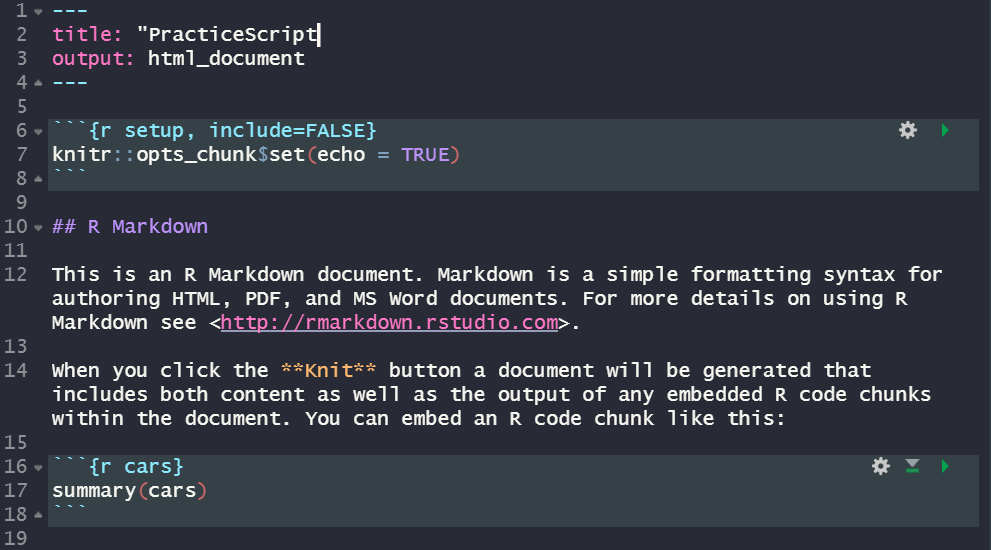
\includegraphics[width=400px]{src/lab01-source-code-chunk-description2}

\begin{itemize}
\tightlist
\item
  \textbf{Exercise 6:} Read the text in the practice script you created.
  Click the button labeled \textbf{Knit}. Save the file name as
  ``PracticeScript''. Compare the file that is generated when you hit
  ``Knit'' (it should open in a pop-up window) with the script shown in
  the code editor.

  \begin{itemize}
  \tightlist
  \item
    See Figure 2.1 on this website:
    \url{http://socviz.co/gettingstarted.html}. From Figure 2.1, notice
    what is typed in markdown vs.~what the output looks like.
  \end{itemize}
\item
  \textbf{Exercise 7:} Delete lines 8 through 30 of the practice script
  markdown file. This should leave only the header information (the top
  four lines including the ``---'' at the top and bottom). Knit your
  file and see what appears in the Viewer window.
\item
  \textbf{Exercise 8:} Update the title of your file (line 2) to
  ``Report on wages'' by typing into the source. Then, starting on line
  8 write: ``To calculate my monthly wage, I multiplied the hourly rate
  by the number of hours worked and multiplied this product by the
  number of weeks in a month. Finally, I multiplied by 80\% to account
  for taxes.'' Then knit your file again.
\item
  \textbf{Exercise 9:} Add a code chunk to the file at line 12. To do
  this, click the place in the template you'd like to add your chunk,
  and then click the \textbf{Insert} button and choose R from the
  dropdown menu. The keyboard shortcut for this is
  \texttt{option\ +\ cmd\ +\ i} on Mac OS and
  \texttt{Ctrl\ +\ Alt\ +\ i} on PC.
\item
  \textbf{Exercise 10:} Write the code
  \texttt{monthly\_wage\ \textless{}-\ 20\ *\ 15\ *\ 4\ *\ 0.8} inside
  the code chunk. Name the code chunk ``calculate-wage'' (see the image
  above to remind yourself how to name the code chunk).
\item
  \textbf{Exercise 11:} On the next line (inside the code chunk) write
  \texttt{monthly\_wage}. When we execute this line, we are asking R to
  display the value that we assigned to the variable
  \texttt{monthly\_wage}. Execute the code chunk by pressing its green
  arrow or placing your cursor on the line of code and hitting
  \texttt{cmd\ +\ enter} on Mac or \texttt{Ctrl\ +\ enter} on PC.
\end{itemize}

\setlength{\leftskip}{0pt}

\textbf{Pane 4. Files/Plots/Packages/Help/Viewer} These tabs are all
useful! The file tab is a basic file viewer. What files are in your
folder? The Plots tab displays any plots you've created using code
executed in the console. The packages tab shows you the R packages
installed (as a list) and those loaded are checked off. We will talk
more about R packages in the next lab. The Help tab is used to search
the help files. The Viewer tab is used to view other types of output
(often html output), like the file we created when we knit the R
markdown file.

\subsubsection{What is an R package?}\label{what-is-an-r-package}

\begin{itemize}
\tightlist
\item
  An R package is a set of \textbf{functions} that someone has put
  together. For example, the package \texttt{ggplot2} is a set of
  functions to make plots, the package \texttt{dplyr} is a set of
  functions to manipulate datasets, such as functions to rename and
  create new variables.
\item
  When you load R, a basic set of packages are loaded. R developers have
  created more than 10,000 additional packages that you can download
  from \textbf{CRAN} (The Comprehensive R Archive Network), the main
  repository of R packages.
\end{itemize}

On Datahub, we have already installed the package \texttt{dplyr} and
\texttt{ggplot2} to use during the course. We just need to load the
packages using the \texttt{library()} function:

\begin{Shaded}
\begin{Highlighting}[]
\FunctionTok{library}\NormalTok{(dplyr)}
\FunctionTok{library}\NormalTok{(ggplot2)}
\end{Highlighting}
\end{Shaded}

You can identify a function because it will always end with a set of
round brackets \texttt{()}. Another name for \textbf{function} is
\textbf{command}. \texttt{library(dplyr)} is a \textbf{function} call
with one argument, \texttt{dplyr}. The \textbf{argument} of the
\textbf{function} is inside the round brackets. Many functions take
multiple arguments. Here, we are using the \texttt{library()} function
to load the \texttt{dplyr} package on the first line and the
\texttt{ggplot2} package on the second line.

\subsubsection{What happens when you load a
package?}\label{what-happens-when-you-load-a-package}

Click the packages tab and scroll down to the package name that you
loaded. It should now be checked to indicate that it is loaded. Sometime
when you load a package, a message will display. You don't need to worry
about understanding these messages for now, but here is a description if
you're interested (don't worry if you don't understand, it isn't
important right now and will make more sense as you learn R): - Red
output (called messages) tell you that the package is being attached
(i.e., loaded). It also lists objects that are \textbf{masked} from
other packages. This means that R already had loaded packages called
\texttt{stats} and \texttt{base} and they have functions with the same
names as functions in the\texttt{dplyr} package. Now that we loaded
\texttt{dplyr}, its functions take precedence. If we want to use the
\texttt{filter()} function from the \texttt{stats} package we have to
write \texttt{stats::filter()}, where the package name preceding the
double colons tells you which version of the function you want to use.

\subsubsection{Using the autograder}\label{using-the-autograder}

Problem set and lab questions are evaluated using an autograder. We've
written a series of test cases and checkpoints that test the correctness
of your code and allows you to check your work and receive automated
real-time feedback on your answers.

Now let's try solving a problem. In your assignments, you will be given
a prompt and asked to code the answer and assign it to an object. Do not
change the name of this object. \textbf{For this problem, set
\texttt{p1} to a mathematical expression that evaluates to 5.} You'll
often get starter code that will look like this:

\begin{Shaded}
\begin{Highlighting}[]
\CommentTok{\# Your answer must be stored in the object p1}
\NormalTok{p1 }\OtherTok{\textless{}{-}} \ConstantTok{NULL} \CommentTok{\# YOUR CODE HERE (EXAMPLE ONLY)}
\end{Highlighting}
\end{Shaded}

As you work on the problem, replace the text
\texttt{NULL\ \#\ YOUR\ CODE\ HERE} with your solution to the problem.
Running \texttt{.\ =\ ottr::check("tests/p1.R")} will then tell you if
you're right or wrong, and sometimes provide helpful hints. Let's try.

\begin{Shaded}
\begin{Highlighting}[]
\NormalTok{p1 }\OtherTok{\textless{}{-}} \DecValTok{5}
\end{Highlighting}
\end{Shaded}

\begin{Shaded}
\begin{Highlighting}[]
\NormalTok{. }\OtherTok{=}\NormalTok{ ottr}\SpecialCharTok{::}\FunctionTok{check}\NormalTok{(}\StringTok{"tests/p1.R"}\NormalTok{)}
\end{Highlighting}
\end{Shaded}

\begin{verbatim}
## All tests passed!
\end{verbatim}

When you enter the correct answer,
\texttt{.\ =\ ottr::check("tests/p1.R")} should tell you all checkpoints
passed, and all tests pass for that problem. Now\ldots{} what if we
don't know how to follow directions? Let's see what happens when you
enter in a wrong answer. Run the following chunk in order and observe
their output.

\begin{Shaded}
\begin{Highlighting}[]
\CommentTok{\# This is a WRONG NUMERIC answer. Change it back to 5 afterwards to compare the autograder response!}
\NormalTok{p2 }\OtherTok{\textless{}{-}} \DecValTok{5}
\end{Highlighting}
\end{Shaded}

\begin{Shaded}
\begin{Highlighting}[]
\NormalTok{. }\OtherTok{=}\NormalTok{ ottr}\SpecialCharTok{::}\FunctionTok{check}\NormalTok{(}\StringTok{"tests/p2.R"}\NormalTok{)}
\end{Highlighting}
\end{Shaded}

\begin{verbatim}
## Test p2 - 1 passed
\end{verbatim}

You'll also run into problems that will ask you to explain your answer
in a couple of sentences, like the problem below. Simply replace the
line \texttt{\_Type\ your\ answer\ here,\ replacing\ this\ text.\_} with
your answer. You won't see an autograder check for these free-response
questions since they'll be graded by humans.

\textbf{What are you looking forward to most in this course?}

I am looking forward to\ldots{}

\emph{Type your answer here, replacing this text.}

Now, at the end of the assignment, you should go back through and run
each code chunk to be sure you passed all of your tests. On this
assignment, that only means that \texttt{p1} and \texttt{p2} should
equal 5. Go back and change your answers if they are not! One way to
check that works well is to click the grey downward facing arrow in the
right corner of the code chunk. This will run all previous code chunks
so all of your answers are up to date.≠

When you're happy with your work, you can submit your
assignment--without even leaving RStudio! The submission instructions
will be on the last page of every assignment, including this one. Make
sure you don't forget to submit.

\subsubsection{A Note About the
Autograder}\label{a-note-about-the-autograder}

The autograder is meant to be used as a sanity check for your work, not
as an absolute check of correctness. This is because, in the real world,
you won't have an autograder to check your analysis/code\ldots{} unless
you write your own test cases (which is recommended, but we won't be
covering that in this course). However, \textbf{programming is
difficult}, and we want to provide you with the best resources to
succeed so we will write all the test cases in labs. Since the problem
sets are not being collected for credit, we will also write all the test
cases for these. Our goal is that you won't rely too much on the
autograder for the problem sets - you can try out a few things and try
to intuitively solve the problems. Ask lots of questions - we're excited
for you to start the journey of being a data analyst.

Since \textbf{labs} have an emphasis on introductory learning, all test
cases will be provided. This means if you pass the test cases given in
the assignment, you'll receive full credit on the assignment. Because of
this design, each test case will be graded \textbf{all or nothing,}
which means we will not grant credit for partially correct answers.

\subsubsection{Checking Your Grades \&
Regrades}\label{checking-your-grades-regrades}

When your assignment is graded, it'll be released on Gradescope and
you'll be able to see your code online, as well as the score for each
autograded problem and each free-response question.

We know we're not perfect, and sometimes we mess up the test cases on
the autograder, so a correct answer might get graded as incorrect (we
hope this is rare), so we highly encourage you to check your assignment
promptly after grades are released to make sure you get the score you
earned. If you suspect that the autograder might be incorrect, you can
submit a regrade on Gradescope. Per the regrade policy, \textbf{all
assignment regrades will be open for 3 school days after scores are
released} (scores released anytime Sept.~1st means regrades close
Sept.~4th at 11:59pm).

\subsubsection{Resources}\label{resources}

We will do our best to introduce and demonstrate all of the code you
will need for this class. If you would like to study more on your own,
there are many many resources available online. If you have questions
about R or get stuck, please visit office hours or post on Ed. We highly
encourage this to be the first place where you ask for help!

Hadley Wickham and Garrett Grolemund have written a helpful book about R
that is freely available here: \url{https://r4ds.had.co.nz/}

UCLA has a website with many helpful examples here:
\url{https://stats.idre.ucla.edu/r/}

Finally, Google is your best friend. We will show you how to use Google
to ask questions about R. Generally speaking, many answers to your
questions will live on a website called Stack Overflow.

\newpage

\subsubsection{References}\label{references}

These are the materials I referenced to make these slides. You can look
at them but note that I avoided the material that isn't relevant to us
(and might be confusing for newly-minted learners)

\begin{itemize}
\item
  \url{https://www.computerworld.com/article/1533880/beginners-guide-to-r-introduction.html}
\item
  \url{http://alyssafrazee.com/2014/01/02/introducing-R.html}
\end{itemize}

\newpage

\subsubsection{Before you submit}\label{before-you-submit}

You need to create a password for your Gradescope account \textbf{other}
than the CalNet login process:

\begin{enumerate}
\def\labelenumi{\arabic{enumi}.}
\tightlist
\item
  Go to \url{https://www.gradescope.com/login}
\item
  Click ``School Credentials'' in the bottom left
\item
  Click ``CalNet ID''
\item
  Enter your CalNet ID credentials to log in
\item
  Click on ``Account'' in bottom left select ``Edit Account''
\item
  Create a password and select ``Save Changes''
\end{enumerate}

\textbf{It is important to select ``Save Changes'' so your new password
stays saved.}

\subsubsection{Submission}\label{submission}

For assignments in this class, you'll be submitting using the
\textbf{Terminal} tab in the pane below. In order for the submission to
work properly, make sure that:

\begin{enumerate}
\def\labelenumi{\arabic{enumi}.}
\tightlist
\item
  Any image files you add that are needed to knit the file are in the
  \texttt{src} folder and file paths are specified accordingly.
\item
  You \textbf{have not changed the file name} of the assignment.
\item
  The file knits properly.
\end{enumerate}

Once you have checked these items, you can proceed to submit your
assignment.

\begin{enumerate}
\def\labelenumi{\arabic{enumi}.}
\tightlist
\item
  Click on the \textbf{Terminal} tab in the pane below.
\item
  Copy-paste the following line of code into the terminal and press
  enter.
\end{enumerate}

cd; cd ph142-su26/lab/lab01; python3.11 turn\_in.py

\begin{enumerate}
\def\labelenumi{\arabic{enumi}.}
\setcounter{enumi}{2}
\tightlist
\item
  Follow the prompts to enter your Gradescope username and password.
  \textbf{Note: the terminal will not show your password being typed
  out. This is intentional as a security mechanism. Type your password
  as indicated and hit return/enter to submit.}
\item
  If the submission is successful, you should see ``Submission
  successful!'' appear as the output. \textbf{Check your submission on
  the Gradescope website to ensure that the autograder worked properly
  and you received credit for your correct answers. If you think the
  autograder is incorrectly grading your work, please post on piazza!}
\item
  If the submission fails, try to diagnose the issue using the error
  messages--if you have problems, post on Piazza under the post
  ``Datahub Issues''.
\end{enumerate}

The late policy will be strictly enforced, \textbf{no matter the
reason}, including submission issues, so be sure to submit early enough
to have time to diagnose issues if problems arise.

\end{document}
